\documentclass[12pt,a4paper]{article}

\setcounter{secnumdepth}{3}
% USEPACKAGE LISTA
\usepackage[utf8]{inputenc}
\usepackage{amsmath}
\usepackage{mathtools}
\usepackage{marvosym} 
\usepackage{wrapfig}
\usepackage{hyperref}
\usepackage{float}
\usepackage{multicol}
\hypersetup{colorlinks,citecolor=black,filecolor=black,linkcolor=black,urlcolor=black}
\usepackage{pdfpages}
\usepackage{amsfonts}
\usepackage{amssymb}
\usepackage{hyperref}
\usepackage{fancyhdr}
\usepackage{graphicx}
\usepackage[export]{adjustbox}
\usepackage{t1enc}
\usepackage[english]{babel}
\usepackage{bm}
\usepackage{multirow}

\usepackage{booktabs}

\usepackage{pgfplots}
\pgfplotsset{height = 10cm, width=15cm,compat=1.9}

% \usepackage[usenames,dvipsnames]{xcolor}
\usepackage[left=2cm,right=2cm,top=2cm,bottom=2cm]{geometry}

\usepackage{listings} % For inline code listings
\usepackage{xcolor}   % For custom colors in listings

% Define Python code style for listings
\lstdefinestyle{python}{
    language=Python,
    basicstyle=\ttfamily\small,
    keywordstyle=\color{blue}\bfseries,
    stringstyle=\color{red},
    commentstyle=\color{gray},
    showstringspaces=false,
    frame=single,
    numbers=left,
    numberstyle=\tiny\color{gray},
    breaklines=true,
    breakatwhitespace=true,
    tabsize=4
}

\setlength{\parindent}{0pt} % bekezdés behúzása
\setlength{\parskip}{0em}   % bekezdések közti távolság
\pagestyle{fancy}
\fancyhf{}


% --> disable section num
% \setcounter{secnumdepth}{0}



\title{Finite elastic-plastic deformations\\(BMEGEMMDKPL)\\II. Homework}
\author{Szász Zsolt\\KRCH5Q}
\date{May 3, 2025}

\lhead{Szász Zsolt\\KRCH5Q}
\chead{}
\rhead{Finite elastic-plastic deformations\\II. Homework}
\cfoot{\thepage. page}

% ITT KEZDŐDIK A DOKUMENTUM



\begin{document}


\maketitle{}
\newpage

\section{Data}

\subsection*{Loading}

We have  an $L$ mm $\times$ $L$ mm $\times$ $L$ mm brick element ($L=1$ mm), shown in Figure \ref{fig:cube}.

\begin{figure}[h]
    \centering
    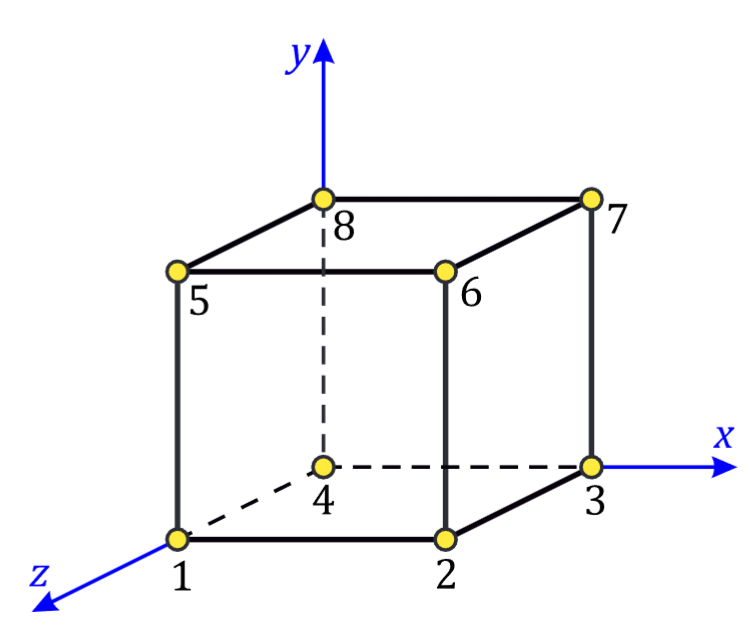
\includegraphics[scale=0.5]{figures/cube.png}
    \caption{Nodal layout of the brick element.}
    \label{fig:cube}
\end{figure}

We have a prescribed displacements on the upper nodes, whicg is defined in the following way

\begin{equation}
    [\boldsymbol{U_1}] = [\boldsymbol{U_2}] = [\boldsymbol{U_3}] = [\boldsymbol{U_4}] = \begin{bmatrix} 0 & 0 & 0 \end{bmatrix}^T,
\end{equation}

\begin{equation}
    [\boldsymbol{U_5}] = [\boldsymbol{U_6}] = [\boldsymbol{U_7}] = [\boldsymbol{U_8}] = \begin{bmatrix} u_x & u_y & 0 \end{bmatrix}^T.
\end{equation}

The time evolution of $u_x$ and $u_y$ can be observed on Figure \ref{fig:displacements}

\begin{figure}[h]
    \centering
    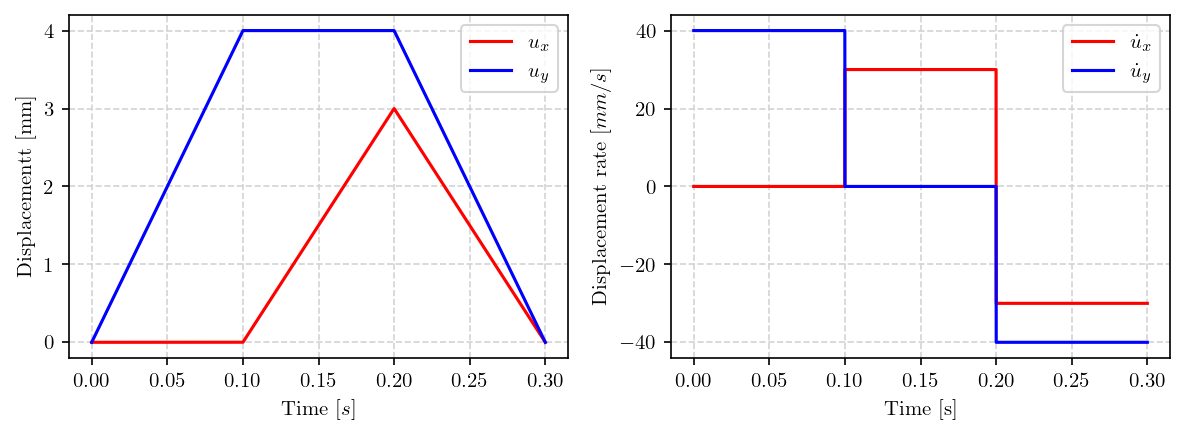
\includegraphics[width=0.8\textwidth]{figures/loading.png}
    \caption{The parameters of the loading}
    \label{fig:displacements}
\end{figure}

From the displacement vectors we can determine the deformations gradient regarding to that motion.

\begin{equation}
    [F] = 
        \begin{bmatrix}
            1 & \frac{u_x}{L} & 0 \\
            0 & 1+\frac{u_y}{L} & 0 \\
            0 & 0 & 1 \\
        \end{bmatrix}.
\end{equation}


The velocity gradient can be calculated with the help of the 

\newpage

\subsection*{Material behaviour}

\newpage


\section*{References}

You can find the detailed code on \href{https://github.com/zsoca000/Finite-elastic-deformations-HW1/blob/main/solution2.ipynb}{\textcolor{blue}{\underline{GitHub}}}.

\end{document}